\chapter{Faceted Web Search}
In this chapter, we define faceted web search and give an overview of our designed FWS system, consisting query facet generation and facet feedback two basic components. Here, we also define related terminologies that will be used throughout this thesis.

\section{Faceted Web Search}
\label{sec:fws}
We define \textbf{Faceted Web Search} as faceted search in the open-domain web setting. Similar to faceted search, FWS system will provide facets when a user issues a web search query. Users can select some terms from the provided facets, which will then be used by the system to adjust the search results to better address the user's information need.
\begin{figure}[ht!]
\centering
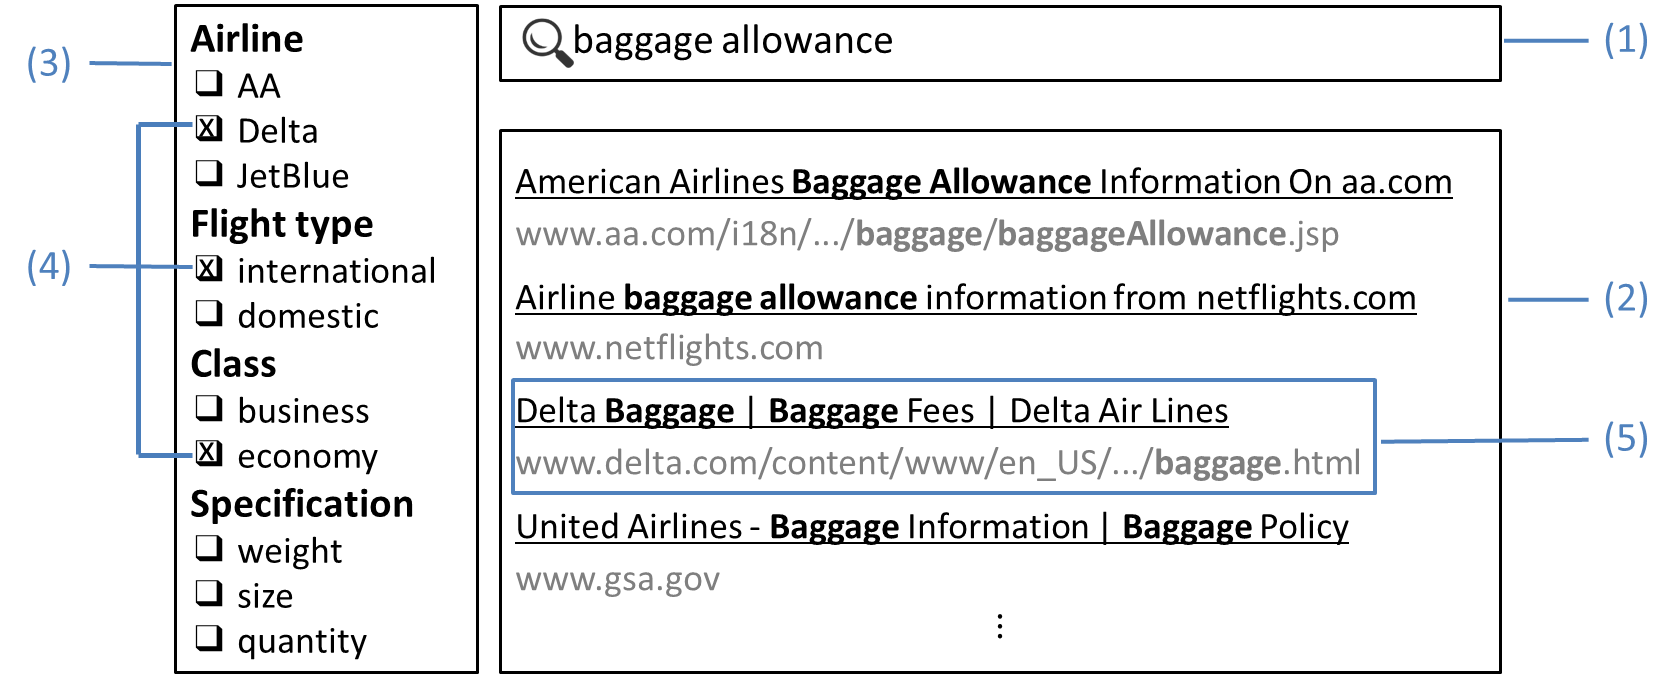
\epsfig{file=figure/fws-example.png,scale=0.45}
%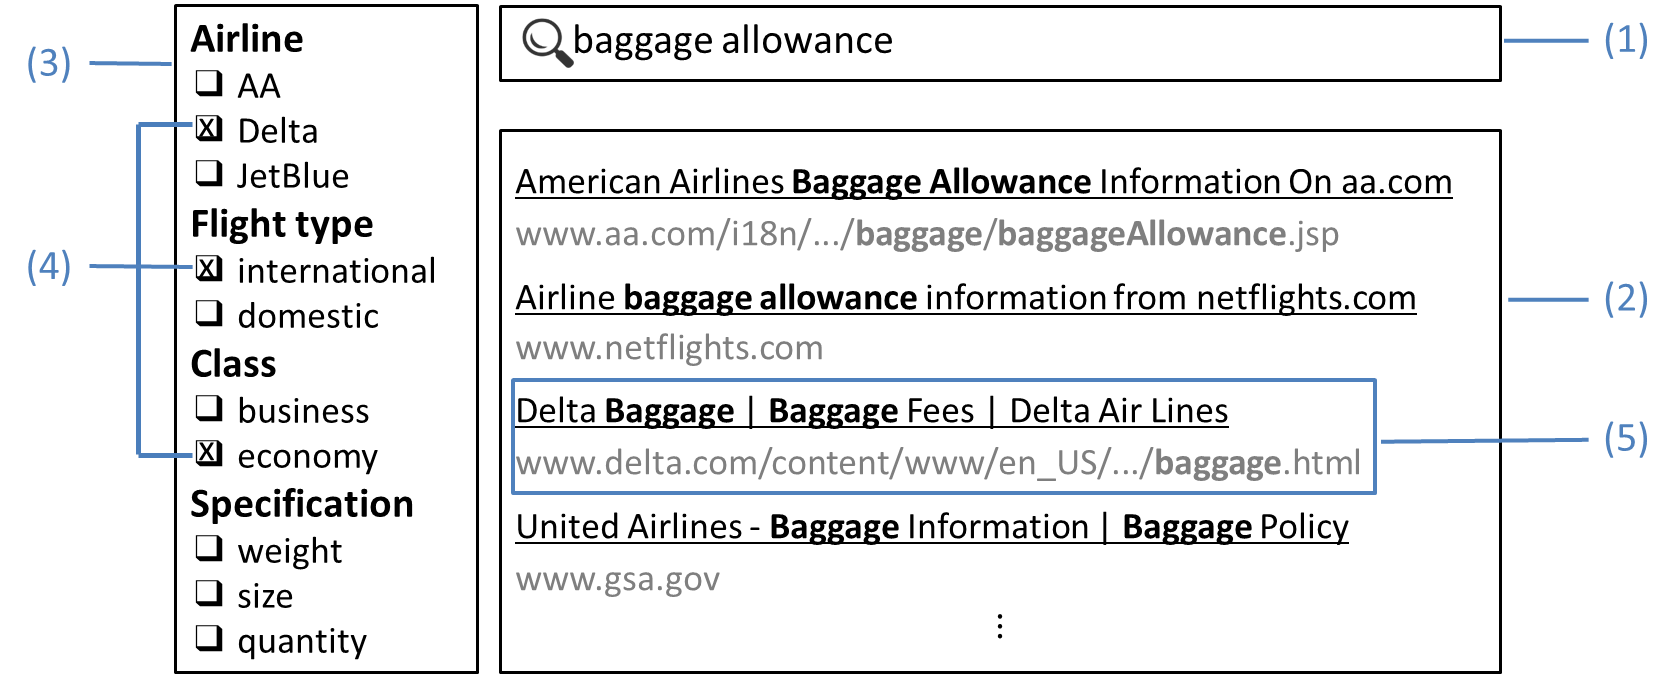
\includegraphics[scale=0.45]{figure/fws-example.png}
\caption{An example case of Faceted Web Search}
\label{fig:fws-example}
\end{figure}
As an example illustrated in Figure~\ref{fig:fws-example}, suppose a user is preparing for an international flight and wants to find baggage allowance information. When the user searches ``baggage allowance'' in an FWS system (step 1 in the figure), in additional to the search result list (step 2), the system will provide a list of facets (step 3), such as a facet for different airlines, \{\textit{Delta}, \textit{JetBlue}, \textit{AA}, ...\}, a facet for different flight types, \{\textit{domestic}, \textit{international}\}, and a facet for different classes, \{\textit{first}, \textit{business}, \textit{economy}\}. When the user selects terms such as ``Delta'', ``international'' and ``economy'' in these facets (step 4), the system can ideally help to bring web documents that provide baggage allowance information for the economy class of Delta international flights to the top of the search results (step 5).

There are two basic components in a FWS system, query facet generation and facet feedback.

\section{Query Facet Generation}
In conventional faceted search, facets are typically generated in advance for an entire corpus~\cite{stoica2007automating,dakka2008automatic} either manually or semi-automatically, and then recommended for particular queries. However, this approach is difficult to be extended for the general web due to its large and heterogeneous nature. To cope with this challenge, we propose \textbf{query facet generation}, a query-dependent approach that generates facets for a particular query instead of the entire corpus (corresponds to step 3 in Figure~\ref{fig:fws-example}). This not only makes the generation problem easier, but also addresses the facet recommendation problem at the same time.

To differentiate with facets in conventional faceted search, we call facets for a particular query \textbf{query facets}. A query facet is a set of coordinate terms -- i.e., terms that share a semantic relationship by being grouped under a more general hypernym (``is a'' relationship), and they succinctly represent different options in a same category that a user can select to refine the issued query. Table~\ref{tab:facetexample} shows query facets for three queries as examples. To illustrate, for the last query \textit{Mars Landing}, three query facets are shown.
\begin{table}[ht!]
\centering
\caption{Query facet examples for three queries}
\label{tab:facetexample}
\begin{tabular}{|l|} \hline
Query 1: baggage allowance \\\hline
Facet 1: AA, Delta, Jetblue,  ... \\
Facet 2: international, domestic \\
Facet 3: first class, business class, economy class \\
Facet 4: weight, size, quantity \\\hhline{|=|}
Query 2: Mr Bean \\\hline
Facet 1: comics, movies, tv, books \\
Facet 2: The Curse of Mr Bean, Mr Bean Goes to Town, ...\\
Facet 3: Rowan Atkinson, Richard Wilson, Jean Rochefort,  ...\\ 
Facet 4: Mr Bean, Irma gobb, Rupert, Hubert, ...\\\hhline{|=|}
Query 3: Mars landing \\\hline
Facet 1: Curiosity, Opportunity, Spirit \\
Facet 2: USA, UK, Soviet Union \\
Facet 3: video, pictures, news \\\hline
\end{tabular}
\end{table}
The first query facet, \{\textit{Curiosity}, \textit{Opportunity}, \textit{Spirit}\}, includes different Mars rovers. The second query facet, \{\textit{USA}, \textit{UK}, \textit{Soviet Union}\}, includes countries relevant to Mars landings. These are both facets where the terms are instances of the same semantic class. 
Somewhat differently, the last facet, \{\textit{video}, \textit{pictures}, \textit{news}\}, includes labels for different query subtopics. These labels can be viewed as instances of a special semantic class, the subtopics of the query \textit{mars landing}. We call the terms inside facets \textbf{facet terms}, which can be single words (e.g. ``international'', ``domestic'' in Table~\ref{tab:facetexample}) or phrases (e.g. ``first class'', ``business class'' in Table~\ref{tab:facetexample}). When it is clear from context, we will simply use ``facet'' for ``query facet'', and ``term'' for ``facet term'' for convenience.

While a variety of different resources can be used for query facet generation, such as a query log, anchor text, taxonomy and social folksonomy, we develop the first approach for query facet generation by extracting query facets from top search results for issued queries, which will be described in detail in Chapter~\ref{ch:facet}

\section{Facet Feedback}
\textbf{Facet feedback} is to use users' selections on the facets to adjust (filter or re-rank) the search results (corresponds to step 5 in Figure~\ref{fig:fws-example}). We call the facet terms users selected \textbf{feedback terms}, and facets that contain feedback terms \textbf{feedback facets}. We investigate both Boolean filtering and soft ranking models for facet feedback, which will be described in detail in Chapter~\ref{ch:feedback}